\documentclass{article}
\usepackage[top=0.5cm, bottom=0.5cm, left=1cm, right=1cm, marginparwidth=0.75cm]{geometry}

\usepackage{graphicx} % Required for inserting images

\usepackage{tikz}
\usetikzlibrary{arrows.meta, decorations.pathmorphing}

\usepackage{caption}
\usepackage{subcaption}

\title{Minimisation de la distance maximale entre deux particules}
\author{Ilyes BENNANI - Nathan LE CORRE - Fenril GERNÉ}
\date{April 2026}

\begin{document}

\maketitle

\section{Problème étudié}

On dispose d'un environnement $e$ et d'une durée $T$. Dans une simulation de $e$ qui durerait au moins $T$ secondes, on cherche à minimiser la distance maximale entre deux particules de $e$, lors de la première itération qui dépasse (au sens large) les $T$ secondes.
Pour ce faire, on se donne le droit de modifier les positions et vitesses initiales des particules de $e$.

\section{Description de l'innovation}

On réfléchit à partir de l'état final. On cherche à placer les particules de la manière la plus compacte possible (mais de sorte à ce qu'il soit possible d'accéder à cet état en T secondes).
On cherche ensuite à faire la simulation à l'envers pour trouver l'état initial correspondant.
Le principal défi lié à cette approche est qu'à chaque collision dans une simulation, de l'information est perdue : celle de la vitesse précédente des particules engagées dans la collision.

On cherche alors à ce que toutes les collisions aient lieu dans un même contexte prédictible : celui de 2 particules se déplaçant sur une même droite.

Pour se faire, on place les particules sur une grille d'interstice à peine supérieur à $r$, et de sorte à remplir la forme qui maximise l'aire pour un diamètre minimal : le disque.

On impose pour que ce modèle fonctionne $2\times dl < r$, où $dl = dt\times 1m\cdot s^{-1}$. Dans le cas contraire, 2 particules qui se foncent dessus pourraient se dépasser AVANT d'entrer en collision pendant la simulation inverse, menant alors à un état inaccessible.

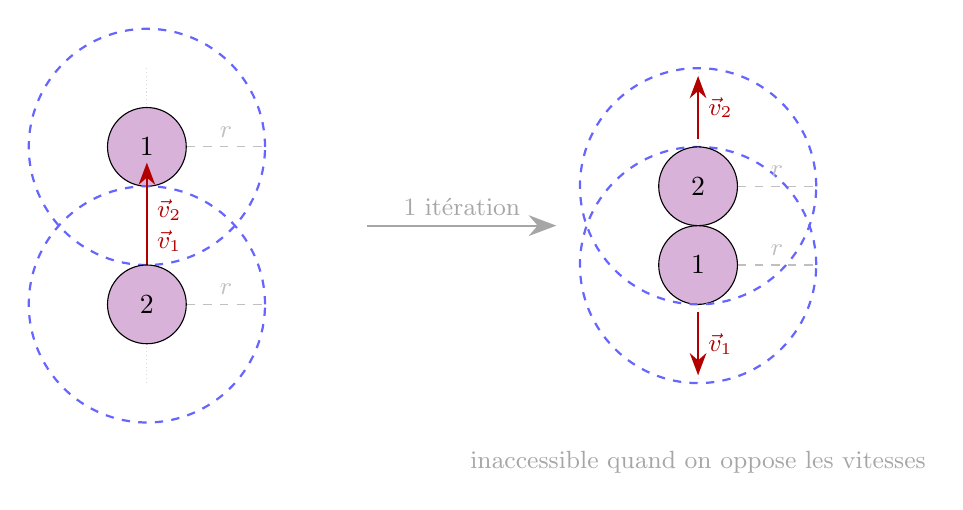
\begin{tikzpicture}[
  particle/.style={circle, draw, fill=violet!30, minimum size=1cm, inner sep=0pt},
  velocity/.style={-{Stealth[length=8pt]}, thick, red!70!black},
  dashed circle/.style={dashed, blue!60, thick},
  radius/.style={dashed, gray!50, thin},
  transition/.style={-{Stealth[length=10pt]}, thick, gray!70},
]

  % ─── État initial (gauche) ───────────────────────────

  % Axe vertical discret
  \draw[gray!30, densely dotted] (0, -2) -- (0, 2);

  % Particule 1 (en haut)
  \node[particle] (p1) at (0, 1)  {$1$};
  \draw[dashed circle] (p1) circle (1.5cm);
  \draw[radius] (p1) -- node[above, midway, font=\small\itshape]{$r$} ++(1.5, 0);
  \draw[velocity] (p1) ++(0,-0.6) -- ++(0,-1.2)
    node[right, midway, font=\small\itshape]{$\vec{v}_1$};

  % Particule 2 (en bas)
  \node[particle] (p2) at (0, -1) {$2$};
  \draw[dashed circle] (p2) circle (1.5cm);
  \draw[radius] (p2) -- node[above, midway, font=\small\itshape]{$r$} ++(1.5, 0);
  \draw[velocity] (p2) ++(0, 0.6) -- ++(0, 1.2)
    node[right, midway, font=\small\itshape]{$\vec{v}_2$};

  % ─── Flèche de transition ────────────────────────────

  \draw[transition] (2.8, 0) -- node[above, font=\small]{1 itération} ++(2.4, 0);

  % ─── État final (droite) ─────────────────────────────

  % Axe vertical discret
  \draw[gray!30, densely dotted] (7, -2) -- (7, 2);

  % Particule 1 maintenant en bas (elle a continué vers le bas)
  \node[particle] (p1f) at (7, -0.5) {$1$};
  \draw[dashed circle] (p1f) circle (1.5cm);
  \draw[radius] (p1f) -- node[above, midway, font=\small\itshape]{$r$} ++(1.5, 0);
  \draw[velocity] (p1f) ++(0,-0.6) -- ++(0,-0.8)
    node[right, midway, font=\small\itshape]{$\vec{v}_1$};

  % Particule 2 maintenant en haut (elle a continué vers le haut)
  \node[particle] (p2f) at (7,  0.5) {$2$};
  \draw[dashed circle] (p2f) circle (1.5cm);
  \draw[radius] (p2f) -- node[above, midway, font=\small\itshape]{$r$} ++(1.5, 0);
  \draw[velocity] (p2f) ++(0, 0.6) -- ++(0, 0.8)
    node[right, midway, font=\small\itshape]{$\vec{v}_2$};

  % Label temporel
  \node[font=\small, gray!70] at (7, -3) {inaccessible quand on oppose les vitesses};

\end{tikzpicture}


Le cas $2 \times dl \ge r$ est traité de manière assez peu intéressante.

\section{Protocole expérimental}


Nous allons maintenant faire des tests sur notre innovation.
\\
Ces tests seront effectués avec un environnement fixe : $h = w = 100$, $dt = 0.1$, $r = 5$.
\\[5 mm]
On initialise un environnement avec ces données, et le nombre de particules souhaitées.
\\
Ensuite, on exécute le code de l'innovation, et on étudie l'environnement obtenu juste après.
\\[5 mm]
Pour évaluer l'efficacité du code, il faut évaluer la plus grande distance entre deux particules.
\\
Nous nous contenterons simplement d'évaluer chacune des distances, pour ainsi prendre celle qui est minimale.
\\[5 mm]
Nous avons ainsi une fonction de test pour un nombre de particules donné, et un $T$ donné, mais nous souhaiterons obtenir plusieurs données pour pouvoir les étudier.
\\
Ainsi, pour un $T$ donné, nous calculerons 100 données avec comme nombre de particules 10, puis 20, puis 30, jusqu'à 1 000.
\\
Pour chaque itération, nous calculerons la distance maximale obtenue, ainsi que le temps d'exécution de l'innovation.
\\[5 mm] 
Ces valeurs seront écrites dans un fichier .csv dont le nom est "test\_[$T$].csv".
\\
Il y aura 3 colonnes de valeurs :
\begin{enumerate}
    \item Le nombre de particules.
    \item La distance maximale calculée entre deux particules.
    \item Le temps d'exécution.
\end{enumerate}

Nous ferons les tests avec les valeurs de $T$ suivantes : 1, 10, 50 et 100.

\section{Résultats}

\begin{figure}[hb]
    \begin{subfigure}{0.5\linewidth}
        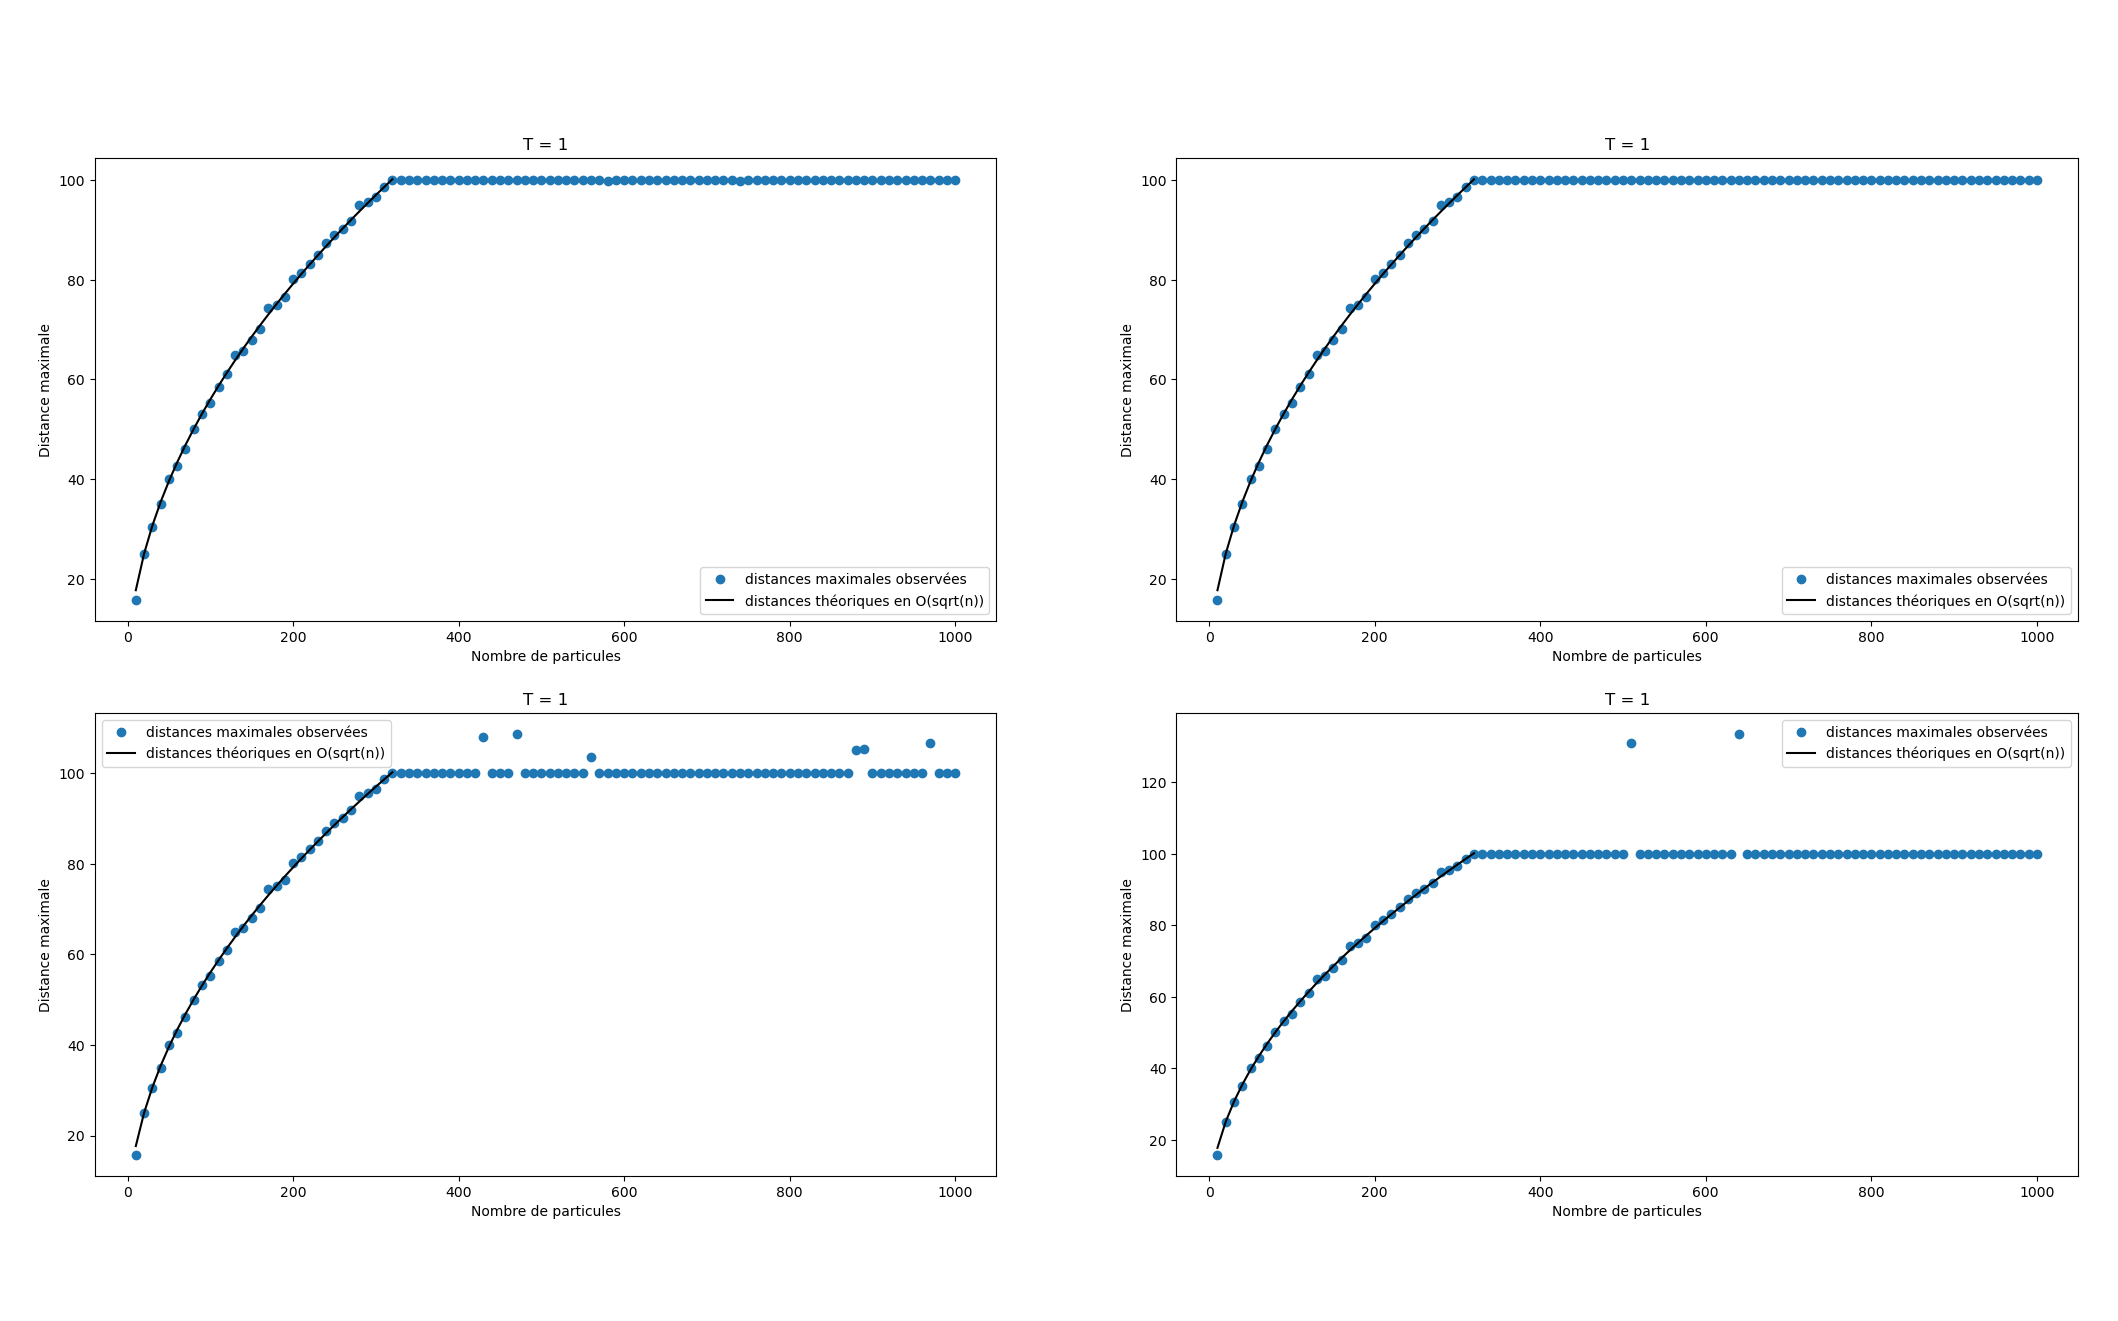
\includegraphics[width=\linewidth]{Figure_1.png}
    \end{subfigure}%
    \begin{subfigure}{0.5\linewidth}
        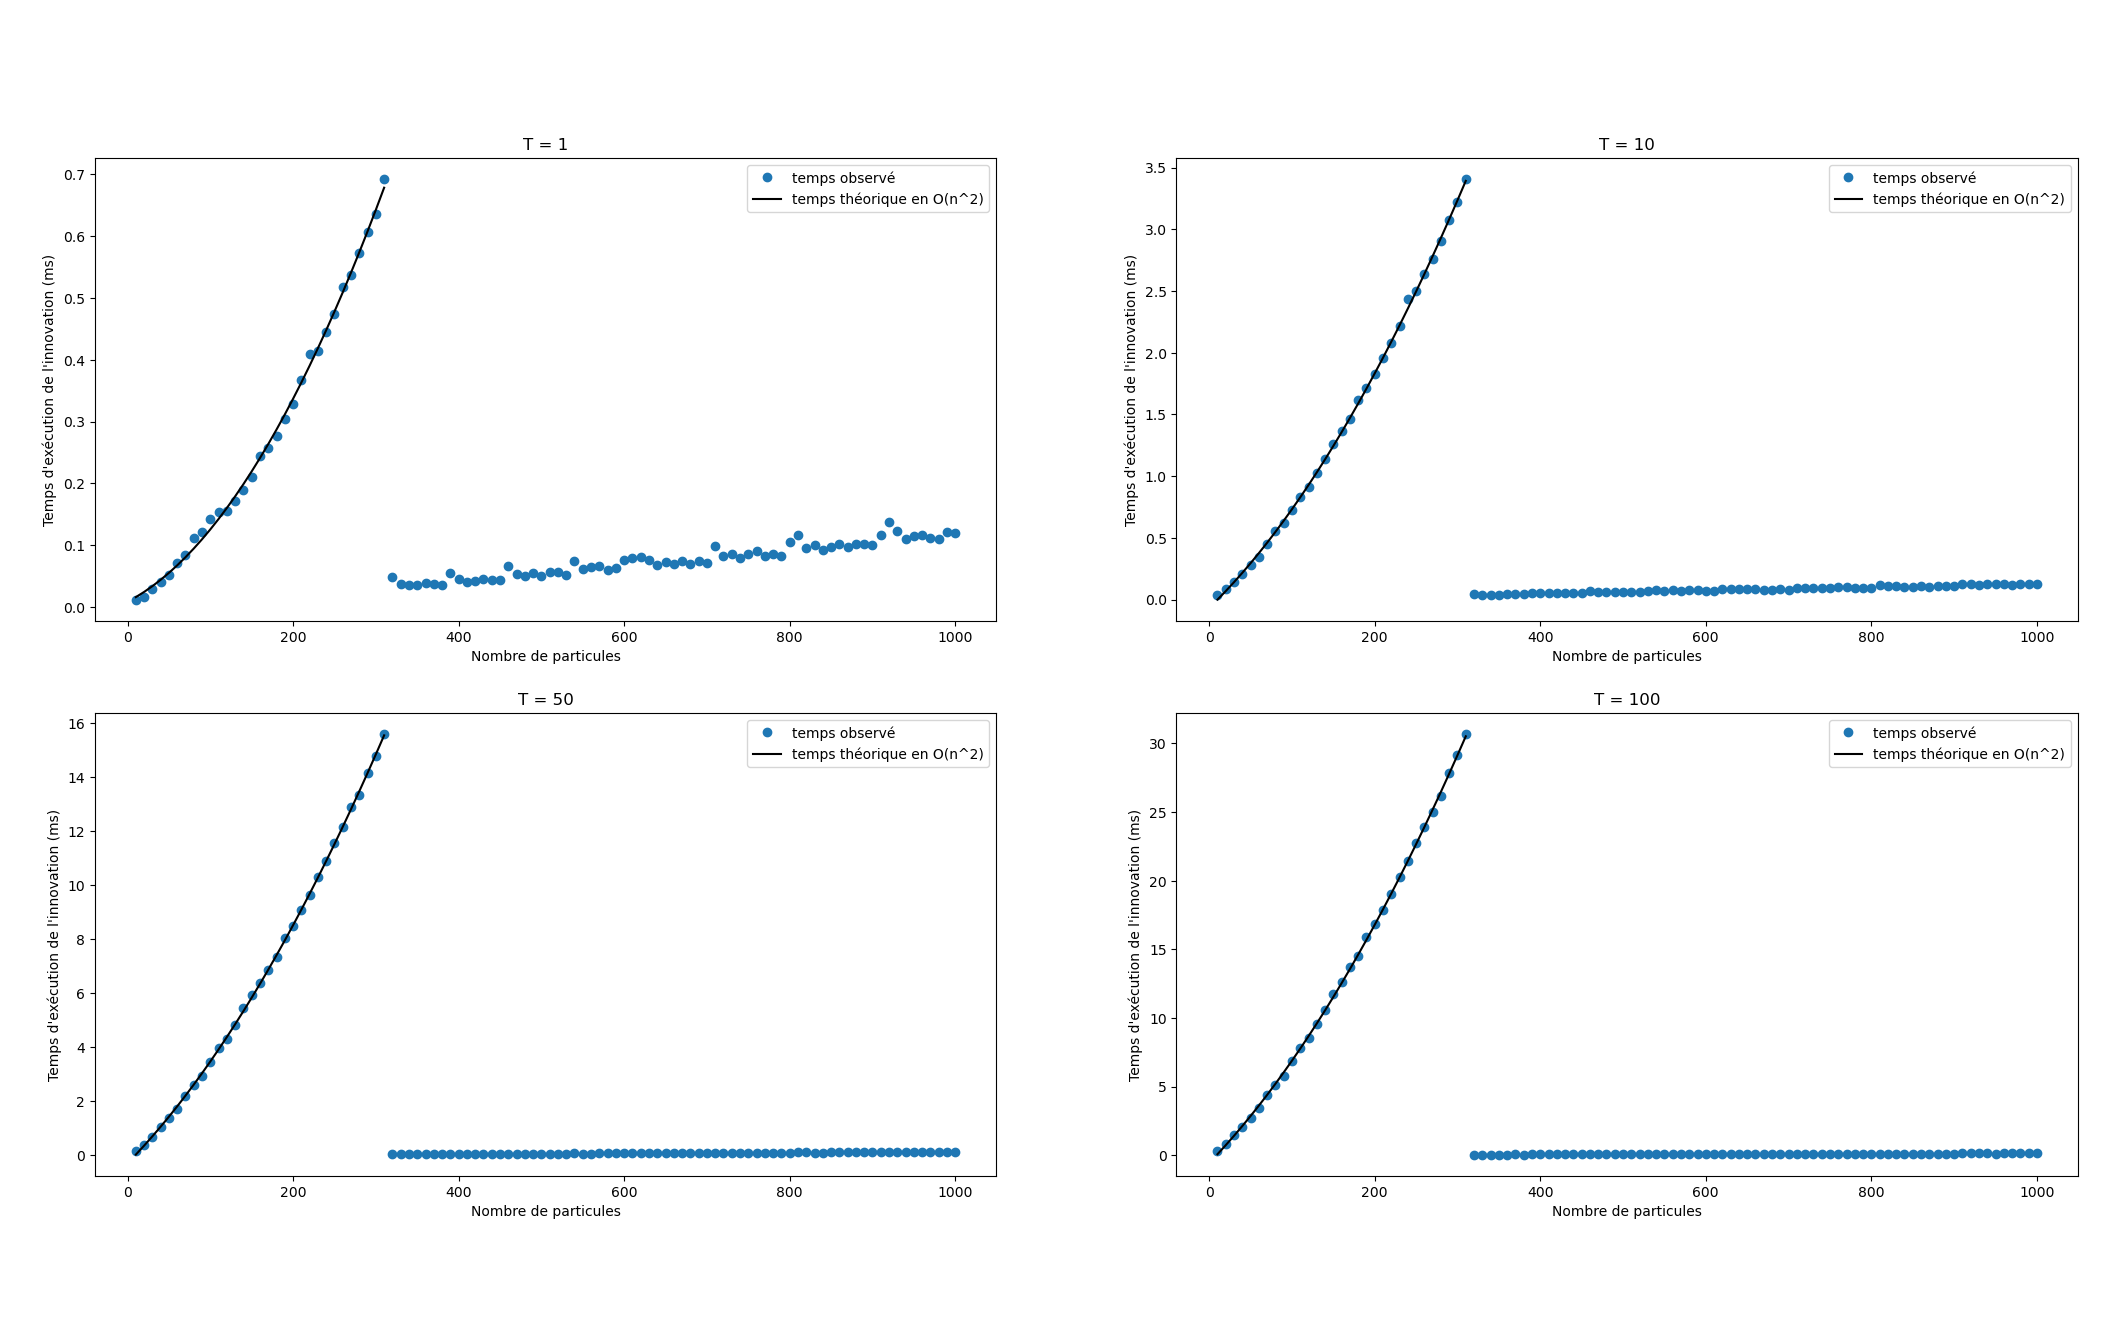
\includegraphics[width=\linewidth]{Figure_2.png}
    \end{subfigure}
    \caption{Distance maximale entre particules et temps d'exécution en fonction du nombre de particules}
\end{figure}

Sur le premier graphique sont représentées les distances maximales en fonction du nombre de particules.\\
On remarque que la distance maximale est en $\Theta(\sqrt n)$ jusqu'à 310 particules ; c'est le rayon de notre cercle.
À partir de 320 particules on change d'algorithme car notre cercle dépasserait de l'environnement, on place les particules en lignes en bas (ou sur le côté dépendant de l'environnement) ; les particules restent sur cette ligne si il n'y a pas de collisions parfaitement centrées, celles-ci étant aléatoires. C'est pour cela qu'on observe à partir de 320 particules une distance maximale constante à 100 sauf dans quelque cas de collisions centrées qui sont d'autant plus probable d'arriver que la simulation dure longtemps.\\
\\
Sur le second graphique sont représentés les temps d'exécution de l'innovation en fonction du nombre de particules.\\
La complexité en temps de l'innovation est en $O(n^2)$ tant qu'on n'utilise pas l'algorithme simple, c'est la complexité théorique de l'algorithme.
Après cela on place linéairement les particules, on devrait observer une complexité linéaire ce qui est particulièrement remarquable pour $T=1$ bien qu'il y ait des fluctuations assez importante pour une raison inconnue (certainement que le moment où l'innovation détecte qu'elle doit utiliser l'algorithme simple dépend de l'indice de la première particule hors de l'environnement ce qui varie fortement avec n).\\
Dans le pire cas testé (310 particules pendant 100 secondes) on a un temps d'exécution d'environ 31ms sur un AMD Ryzen™ 7 7800X3D.


\section{Conclusion}
L'innovation est très performante dans le cas où l'on peut placer les particules dans un cercle sans qu'elles interagissent entre elles. On atteint alors une distance en $\Theta(\sqrt n)$.\\
Dans les autres cas notamment si $2dl \ge r$ on arrive à obtenir une distance maximale constante à $min(h, w)$ la plupart du temps, si deux particules se superposent parfaitement à n'importe quel moment on peut difficilement y faire grand chose.

\end{document}
